% !TEX root = ../main.tex
\begin{comment}
=== Revision log ===
2026-05-08  R. Cappuccio / Claude  (Wave K -- Introduction rewrite)

  Complete rewrite of the Introduction chapter.  The previous version
  (602 lines) contained two standalone mini-reviews (Quantum Computing
  Landscape, Quantum Sensing Landscape), a detailed Thesis Contributions
  section with three figures and per-contribution Key Results / Impact
  paragraphs, and a Methodological Framework section.  All of this
  material either duplicated what the individual chapters already
  provide or anticipated results better left to those chapters.

  The new Introduction (~190 lines of content) follows a leaner
  structure: a short motivation, the unifying thread that connects
  the three contributions, a one-paragraph-per-chapter thesis outline,
  and the Notation and Conventions block (unchanged from Wave E / S6).
  Three figures previously in the Introduction (fig:asq-transmon,
  fig:qcnn_hybrid_architecture / fig:QCNN-with-std-in,
  fig:B_field_scan_in) have been removed; they remain in their
  respective chapters where they are discussed in context.
  The Two Quantum Revolutions figure (fig:revolutions) is retained.

  Labels preserved: ch:introduction, fig:revolutions, sec:notation.
  Labels removed (no external references): sec:motivation, sec:qcomp,
  sec:qsensing, sec:contributions, sec:methodology, sec:thesis_outline,
  fig:asq-transmon, fig:qcnn_hybrid_architecture, fig:QCNN-with-std-in,
  fig:B_field_scan_in, tab:qs-platforms.
\end{comment}

\chapter{Introduction}
\label{ch:introduction}

Quantum technologies have reached the stage at which individual quantum
systems---superconducting circuits, trapped atoms, photonic channels---can be
prepared, controlled, and measured with sufficient fidelity to attempt tasks
that stretch the limits of classical methods.  The maturity of the enabling
hardware and of full software stacks has ushered in what is sometimes called
the second quantum revolution: a transition from passively exploiting quantum
phenomena (the transistor, the laser) to actively engineering coherence and
entanglement for computing and sensing purposes (Fig.~\ref{fig:revolutions}).

\begin{figure}[h!]
  \centering
  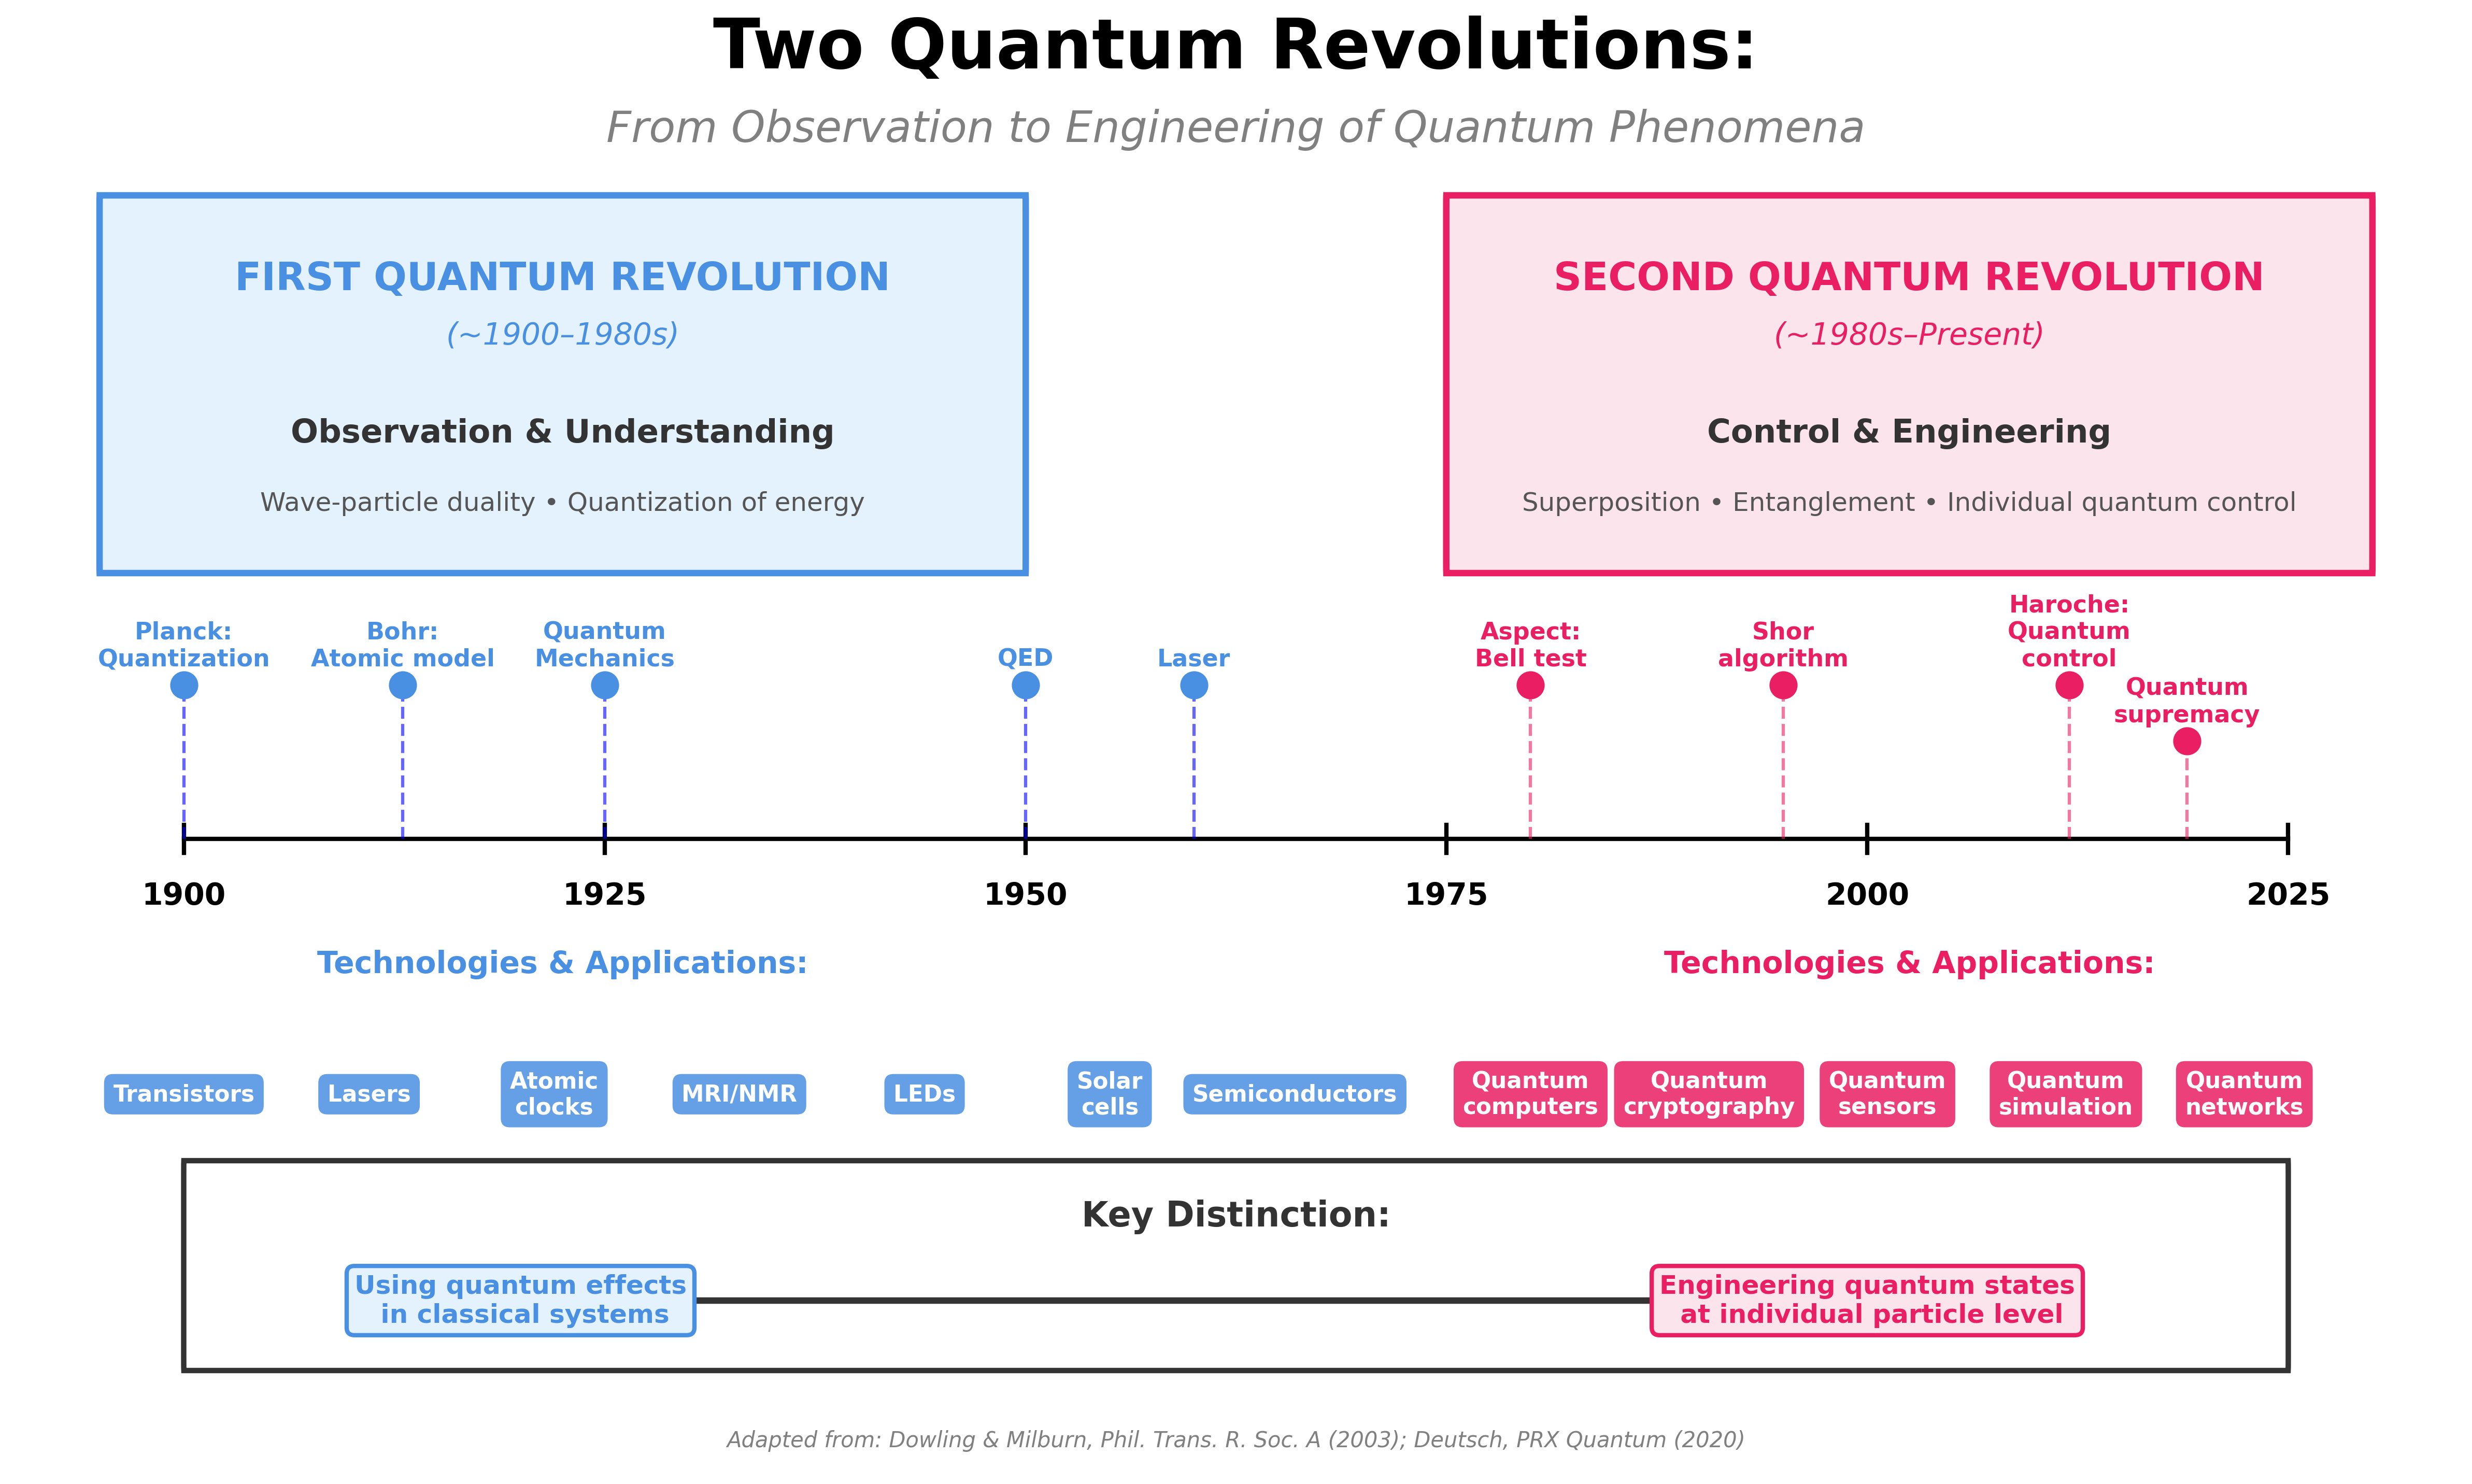
\includegraphics[width=\linewidth]{chapters/in_figures/two_quantum_revolutions_improved_2.png}
  \caption{From observation to engineering of quantum phenomena.
    Adapted from Dowling \& Milburn, \emph{Phil.\ Trans.\ R.\ Soc.\ A}
    (2003) and Deutsch, \emph{PRX Quantum} (2020).}
  \label{fig:revolutions}
\end{figure}

Progress is rapid, yet several practical obstacles remain.  Superconducting
quantum processors require dilution refrigerators operating below
50\,mK---expensive, slow to cool, and difficult to scale.  Hybrid
quantum-classical algorithms show promise for near-term hardware, but
the nature and extent of their advantage over purely classical approaches
is still debated.  Single-photon detectors for fundamental-physics searches
must operate in strong magnetic fields where conventional devices suffer from
prohibitive noise.

This thesis addresses one problem from each of these fronts.  The three
contributions are largely self-contained, but they share a methodological
thread: in each case the investigation is driven by numerical simulation,
used both to explore parameter spaces that are inaccessible experimentally
and to provide quantitative predictions that can guide future hardware
implementations.

\section{Thesis outline}

The remainder of this dissertation is organised as follows.

\paragraph{Chapter~\ref{ch:quantum_hardware} --- Quantum Hardware.}
We develop a system-level design for an asymmetric-SQUID transmon qubit
based on NbN/AlN/NbN Josephson junctions, targeting operation at
$\sim$\,4\,K.  The analysis proceeds in two stages: a baseline at
5.8\,GHz and 20\,mK that anchors the modelling against established
transmon performance, and an elevated-temperature configuration at
300\,GHz and 4\,K where thermal noise, loss mechanisms, and qubit
frequency are jointly examined.  The chapter derives flux-dependent
Hamiltonians for the asymmetric SQUID, characterises its two
flux-insensitive sweet spots, models decoherence, and projects
single- and two-qubit gate fidelities.  The cavity-mediated coupling
between two transmons is analysed in the dispersive regime,
distinguishing transverse exchange from longitudinal cross-Kerr
interactions.

\paragraph{Chapter~\ref{ch:quantum_algorithms} --- Quantum Algorithms.}
We design, train and physically validate a hybrid quantum-classical
convolutional neural network (Q-CNN) for binary satellite-image
classification on a subset of EuroSAT. The architecture inserts a
nine-qubit, eighteen-parameter quanvolutional layer into a classical
convolutional trunk; pixel patches are encoded via rotation angles,
processed through a shallow hardware-efficient entangling block, and
read out as Pauli-$Z$ expectations that feed the classical head.
A multi-seed campaign at $R=10$ independent seeds compares the hybrid
against two purpose-built classical controls --- a structurally
isomorphic matched-capacity baseline (within $0.07\%$ of the hybrid's
parameter count) and a high-capacity reference ($\sim 185\times$ the
hybrid's parameter count) --- with paired Wilcoxon exact tests
documenting a $\sim 2.6$~pp asymptotic-accuracy deficit of the
hybrid against the matched control ($p=2.7\times 10^{-2}$) and a
$\sim 29$~pp training-efficiency advantage at the first epoch on the
same comparison. The chapter also derives a runtime-aware credit-cost
model that links bound-circuit count to a-priori credit consumption,
calibrated against $195$ jobs of the IQM Emerald production campaign,
and closes the loop with a credit-bounded fine-tuning of the
simulator-trained checkpoint on the IQM Emerald 54-qubit
superconducting processor, where parameter-shift gradients restore
$100\%$ validation accuracy in two on-device epochs.

\paragraph{Chapter~\ref{ch:quantum_sensing} --- Quantum Sensing.}
We construct a master-equation model of a Rydberg-atom avalanche
single-photon detector, motivated by the readout requirements of
axion-haloscope experiments.  The model tracks the spatiotemporal
dynamics of a dipole-dipole-driven excitation cascade across a chain
of atoms, and its predictions are examined as a function of an external
magnetic field spanning 0--5\,T.  Sensitivity is analysed through the
quantum Fisher information formalism, and the proposed scheme is
benchmarked against transition-edge sensors, kinetic-inductance
detectors, and superconducting nanowire single-photon detectors.

\paragraph{Chapter~\ref{ch:conclusions} --- Conclusions.}
The final chapter draws together the findings of the three studies,
discusses their limitations, and outlines directions for future work.

% ----------------------------------------------------------------
%  Notation and Conventions
%  (Reactivated and expanded in Wave E, S6 closure -- unchanged.)
% ----------------------------------------------------------------
\section{Notation and Conventions}
\label{sec:notation}

To make the chapters that follow self-contained and to avoid scattering
definitions across the manuscript, we collect here the notational
conventions, the physical constants, and the abbreviations that recur
throughout the thesis.  The list is not meant to be exhaustive:
discipline-specific symbols are introduced where they first appear,
and the present section gathers only those that are referenced in more
than one chapter.

\subsection*{Symbols and conventions}

\begin{itemize}
    \item Quantum states are written in Dirac notation: $\ket{\psi}$ for kets, $\bra{\psi}$ for bras, and $\ket{\psi}\!\bra{\psi}$ for the corresponding rank-one density operator.
    \item Operators carry a hat: $\hat{H}$ for Hamiltonians, $\hat{\rho}$ for density matrices, $\hat{O}$ for a generic observable. Where no ambiguity arises (typically inside long derivations), the hat is dropped.
    \item Pauli operators in the computational basis are denoted $\sigma_x$, $\sigma_y$, $\sigma_z$; the symbols $X$, $Y$, $Z$ denote the same operators in gate notation.
    \item Vectors in Euclidean space are typeset in boldface: $\mathbf{x}$, $\mathbf{E}$, $\mathbf{B}$.
    \item Frequencies and angular frequencies are kept distinct throughout: $f$ denotes a frequency in Hz, while $\omega = 2\pi f$ denotes the corresponding angular frequency in rad/s. Numerical values reported in GHz, MHz, kHz refer to $f$ unless explicitly labelled.
    \item Natural units with $\hbar = 1$ are adopted in formal derivations; SI units are restored whenever numerical results are reported.
    \item Logarithms are base-$2$ in information-theoretic contexts (entropy, mutual information, quantum Fisher information) and natural logarithms elsewhere.
    \item Statistical uncertainties are reported as $95\%$ confidence intervals unless otherwise specified; the analogous interval for fitted parameters is reported at $\pm 1\sigma$.
\end{itemize}

\subsection*{Physical constants}

\begin{itemize}
    \item $k_B$: Boltzmann constant.
    \item $h$: Planck constant; $\hbar = h/(2\pi)$ the reduced Planck constant.
    \item $e$: elementary charge.
    \item $\Phi_0 = h/(2e)$: superconducting magnetic flux quantum.
    \item $c$: speed of light in vacuum.
    \item $\epsilon_0$, $\mu_0$: vacuum permittivity and permeability.
\end{itemize}

\subsection*{Abbreviations}

The following abbreviations recur in more than one chapter. The expansion is given here once; later occurrences use the abbreviation directly, with the expansion repeated only where it improves readability.

\medskip

\noindent\begin{minipage}{\linewidth}
\noindent\textbf{Quantum technologies, broadly.}

\begin{tabularx}{\linewidth}{@{}l@{\hspace{1em}}X@{}}
    \textbf{NISQ} & noisy intermediate-scale quantum (era). \\
    \textbf{QFI}  & quantum Fisher information. \\
    \textbf{QT}   & quantum technology. \\
    \textbf{SQL}  & standard quantum limit. \\
\end{tabularx}
\end{minipage}

\medskip

\noindent\begin{minipage}{\linewidth}
\noindent\textbf{Superconducting hardware.}

\begin{tabularx}{\linewidth}{@{}l@{\hspace{1em}}X@{}}
    \textbf{BCS}     & Bardeen--Cooper--Schrieffer (theory of superconductivity). \\
    \textbf{CMOS}    & complementary metal--oxide--semiconductor (used in the cryo-CMOS variant for control electronics co-located at the cryogenic stage). \\
    \textbf{cQED}    & circuit quantum electrodynamics, the framework for the dispersive coupling of a qubit to a microwave resonator. \\
    \textbf{CQED}    & cavity quantum electrodynamics, the broader atomic-physics framework from which cQED is descended; the two are related but distinct~\cite{blais2021circuit}. \\
    \textbf{DAC}     & digital-to-analogue converter. \\
    \textbf{DRAG}    & derivative removal by adiabatic gate, a pulse-shaping protocol that suppresses leakage to the second excited state of the transmon~\cite{Motzoi2009}. \\
    \textbf{JJ}      & Josephson junction. \\
    \textbf{SQUID}   & superconducting quantum interference device. \\
    \textbf{TLS}     & two-level system (used as a generic term for spurious resonant defects in dielectrics). \\
\end{tabularx}
\end{minipage}

\medskip

\noindent\begin{minipage}{\linewidth}
\noindent\textbf{Quantum machine learning.}

\begin{tabularx}{\linewidth}{@{}l@{\hspace{1em}}X@{}}
    \textbf{ASAP, ALAP} & as-soon-as-possible and as-late-as-possible scheduling policies in transpilation. \\
    \textbf{CNN}        & classical convolutional neural network. \\
    \textbf{PQC}        & parametrised quantum circuit (used interchangeably with VQC; we follow the convention of using PQC for the architectural object and VQC for its training-time use). \\
    \textbf{QCNN}       & hybrid quantum-classical convolutional neural network, the architecture studied in Chapter~\ref{ch:quantum_algorithms}. \\
    \textbf{QML}        & quantum machine learning. \\
    \textbf{SGD}        & stochastic gradient descent. \\
    \textbf{SNR}        & signal-to-noise ratio. \\
    \textbf{VQC}        & variational quantum circuit. \\
\end{tabularx}
\end{minipage}

\medskip

\noindent\begin{minipage}{\linewidth}
\noindent\textbf{Quantum sensing.}

\begin{tabularx}{\linewidth}{@{}l@{\hspace{1em}}X@{}}
    \textbf{EIT}  & electromagnetically induced transparency. \\
    \textbf{SSFI} & state-selective field ionisation, the standard detection technique for cold Rydberg atoms. \\
\end{tabularx}
\end{minipage}
